\subsubsection{Example}

    \begin{itemize}[noitemsep,topsep=0pt]
      \item Starting position: (-1.0, 42.0, 108.0)
      \item End position: (70.0, 56.0, 8.0) 
      \item Euclidean distance from the object: 90.0
      \item Object can be seen: False
      \item Success: False
      \item Object type: crowd
      
    \end{itemize}
    

    \begin{center}
    
\includegraphics[width=0.7\linewidth]{images/GPT4o-CityNew-FS2/20.pdf}
    \end{center}
    

    \begin{center}
    \includegraphics[width=0.7\linewidth]{images/GPT4o-CityNew-FS2/20_sit_awareness.pdf}
    \end{center}
    

    \begin{drama}
    \Character{Benchmark}{re}
    \Character{GPT-4o}{gpt}
    
\respeaks: \( < \)Context\( > \)
    You are in command of a UAV, tasked with finding crowd.
\( < \)/Context\( > \) \texttt{(REST OF THE PROMPT)}
\respeaks: The object you're looking for is similar to this. This is NOT the drone's current view.
\StageDir{\re{} presents \gpt{} with a relevant image}

    \begin{center}
    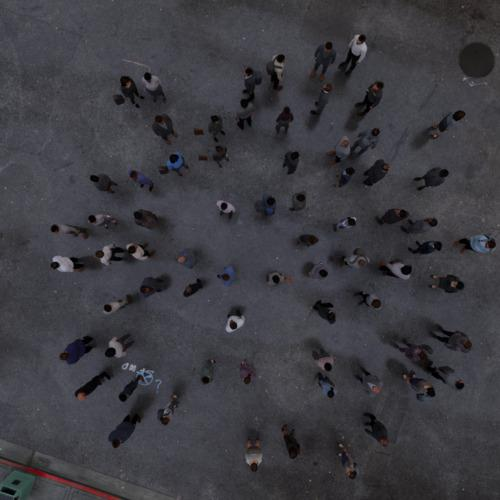
\includegraphics[width=0.5\linewidth]{images/GPT4o-CityNew-FS2/20_0.jpg}
    \end{center}
    
\respeaks: Your current altitude is 108 meters above ground level.
\StageDir{\re{} presents \gpt{} with a relevant image}

    \begin{center}
    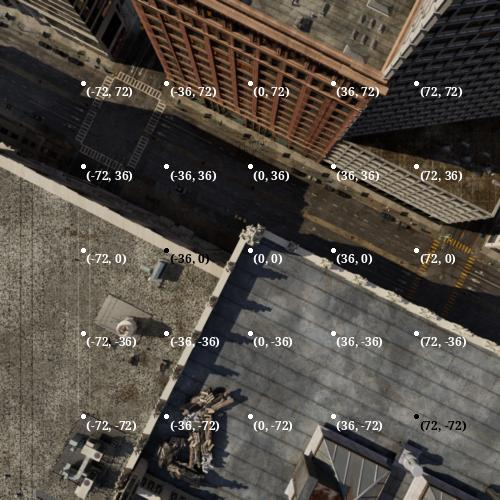
\includegraphics[width=0.5\linewidth]{images/GPT4o-CityNew-FS2/20_1.jpg}
    \end{center}
    
\gptspeaks: \( < \)Reasoning\( > \)From this altitude, I need to lower the drone to get a clearer view and potentially spot the crowd. I will move downward while staying over the central area of the grid for a better observation point.\( < \)/Reasoning\( > \)
\( < \)Action\( > \)(0, 0, -40)\( < \)/Action\( > \)
\respeaks: Emergency stop; you've flown too close to something and would have hit it.
\respeaks: Your current altitude is 83 meters above ground level.
\StageDir{\re{} presents \gpt{} with a relevant image}

    \begin{center}
    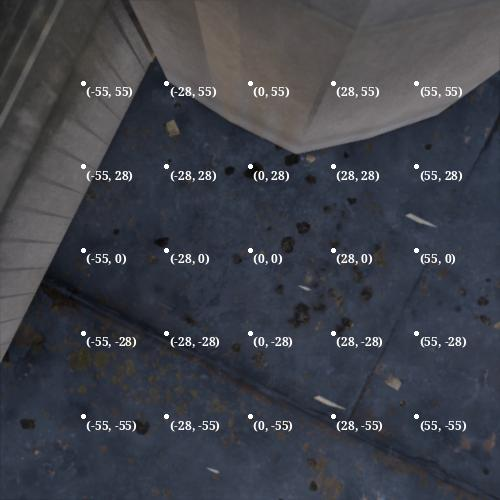
\includegraphics[width=0.5\linewidth]{images/GPT4o-CityNew-FS2/20_2.jpg}
    \end{center}
    
\gptspeaks: \( < \)Reasoning\( > \)I'll move slightly to the open area to the southeast and lower the altitude to continue the search while avoiding obstacles.\( < \)/Reasoning\( > \)
\( < \)Action\( > \)(28, -28, -20)\( < \)/Action\( > \)
\respeaks: Emergency stop; you've flown too close to something and would have hit it.
\respeaks: Your current altitude is 83 meters above ground level.
\StageDir{\re{} presents \gpt{} with a relevant image}

    \begin{center}
    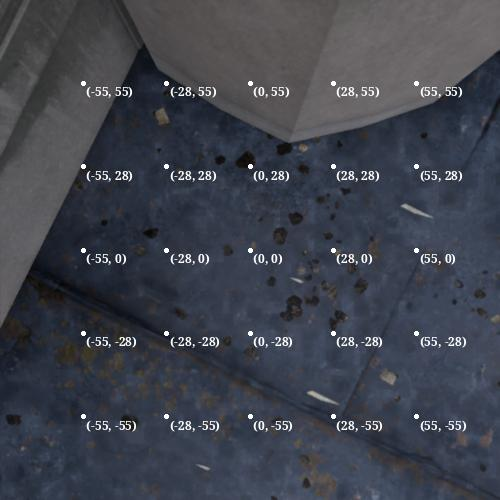
\includegraphics[width=0.5\linewidth]{images/GPT4o-CityNew-FS2/20_3.jpg}
    \end{center}
    
\gptspeaks: \( < \)Reasoning\( > \)I'll adjust my position to the open area to the southwest and lower the altitude to enhance my view, avoiding the building close by.\( < \)/Reasoning\( > \)
\( < \)Action\( > \)(-28, -28, -20)\( < \)/Action\( > \)
\respeaks: Emergency stop; you've flown too close to something and would have hit it.
\respeaks: Your current altitude is 83 meters above ground level.
\StageDir{\re{} presents \gpt{} with a relevant image}

    \begin{center}
    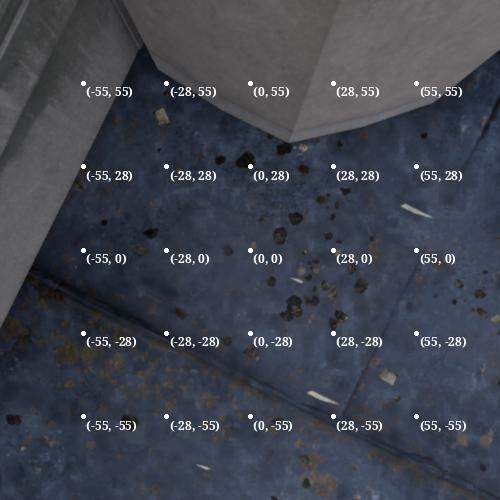
\includegraphics[width=0.5\linewidth]{images/GPT4o-CityNew-FS2/20_4.jpg}
    \end{center}
    
\gptspeaks: \( < \)Reasoning\( > \)I'll move to a clearer spot to the south and decrease altitude, maintaining a safe distance from obstacles.\( < \)/Reasoning\( > \)
\( < \)Action\( > \)(0, -28, -20)\( < \)/Action\( > \)
\respeaks: Emergency stop; you've flown too close to something and would have hit it.
\respeaks: Your current altitude is 83 meters above ground level.
\StageDir{\re{} presents \gpt{} with a relevant image}

    \begin{center}
    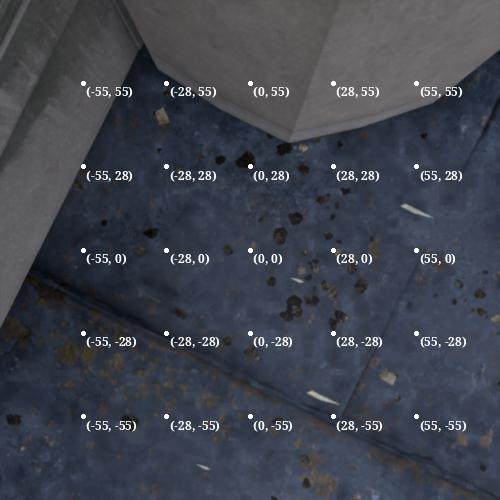
\includegraphics[width=0.5\linewidth]{images/GPT4o-CityNew-FS2/20_5.jpg}
    \end{center}
    
\gptspeaks: \( < \)Reasoning\( > \)I'll move to the southeast this time to avoid obstacles and try to lower the altitude, aiming for an open area.\( < \)/Reasoning\( > \)
\( < \)Action\( > \)(28, -28, -10)\( < \)/Action\( > \)
\respeaks: Emergency stop; you've flown too close to something and would have hit it.
\respeaks: Your current altitude is 83 meters above ground level.
\StageDir{\re{} presents \gpt{} with a relevant image}

    \begin{center}
    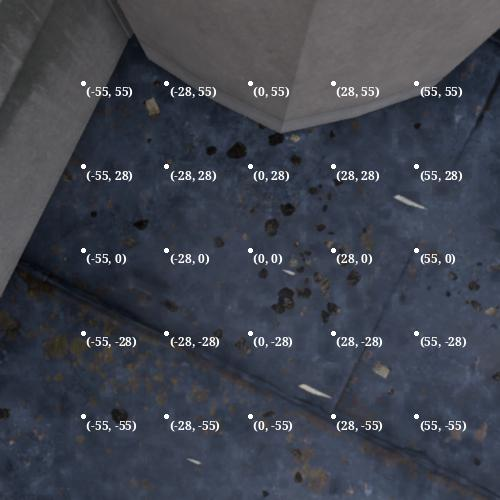
\includegraphics[width=0.5\linewidth]{images/GPT4o-CityNew-FS2/20_6.jpg}
    \end{center}
    
\gptspeaks: \( < \)Reasoning\( > \)I'll move to the east, attempting to find a clear spot and lower the altitude carefully.\( < \)/Reasoning\( > \)
\( < \)Action\( > \)(28, 0, -10)\( < \)/Action\( > \)
\respeaks: Emergency stop; you've flown too close to something and would have hit it.
\respeaks: Your current altitude is 83 meters above ground level.
\StageDir{\re{} presents \gpt{} with a relevant image}

    \begin{center}
    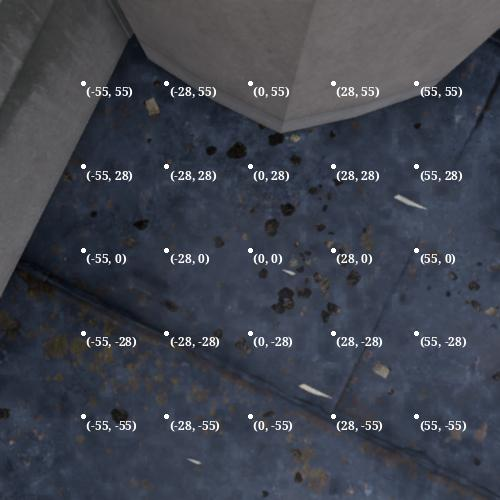
\includegraphics[width=0.5\linewidth]{images/GPT4o-CityNew-FS2/20_7.jpg}
    \end{center}
    
\gptspeaks: \( < \)Reasoning\( > \)I'll ascend slightly to avoid obstacles and move to the southeast to find a clearer view.\( < \)/Reasoning\( > \)
\( < \)Action\( > \)(28, -28, 10)\( < \)/Action\( > \)
\respeaks: Your current altitude is 93 meters above ground level.
\StageDir{\re{} presents \gpt{} with a relevant image}

    \begin{center}
    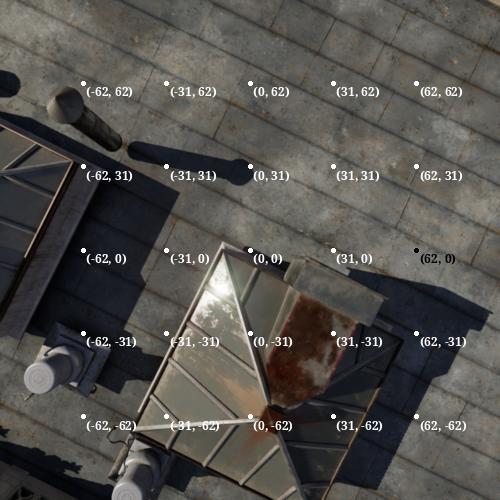
\includegraphics[width=0.5\linewidth]{images/GPT4o-CityNew-FS2/20_8.jpg}
    \end{center}
    
\gptspeaks: \( < \)Reasoning\( > \)I'll continue to move southeast and descend to get a better view over the open area.\( < \)/Reasoning\( > \)
\( < \)Action\( > \)(31, -31, -20)\( < \)/Action\( > \)
\respeaks: Emergency stop; you've flown too close to something and would have hit it.
\respeaks: Your current altitude is 83 meters above ground level.
\StageDir{\re{} presents \gpt{} with a relevant image}

    \begin{center}
    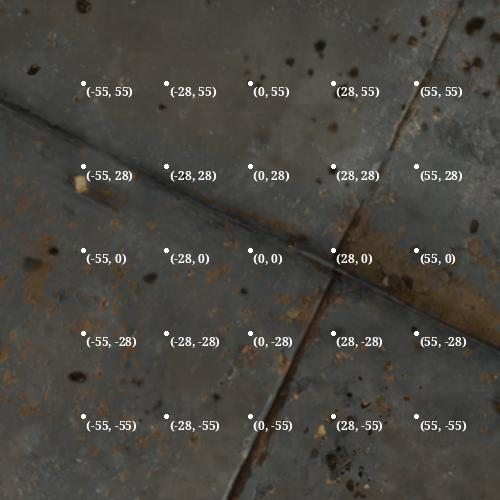
\includegraphics[width=0.5\linewidth]{images/GPT4o-CityNew-FS2/20_9.jpg}
    \end{center}
    
\gptspeaks: \( < \)Reasoning\( > \)I'll move a bit to the east to find a clearer spot and then descend carefully to improve my view.\( < \)/Reasoning\( > \)
\( < \)Action\( > \)(28, 0, -20)\( < \)/Action\( > \)
\respeaks: Emergency stop; you've flown too close to something and would have hit it.
\respeaks: Your current altitude is 83 meters above ground level.
\StageDir{\re{} presents \gpt{} with a relevant image}

    \begin{center}
    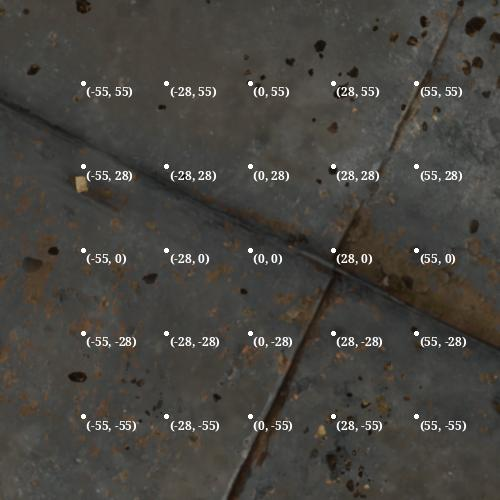
\includegraphics[width=0.5\linewidth]{images/GPT4o-CityNew-FS2/20_10.jpg}
    \end{center}
    
\gptspeaks: \( < \)Reasoning\( > \)I'll move to the north to avoid obstacles and descend slightly to improve visibility.\( < \)/Reasoning\( > \)
\( < \)Action\( > \)(0, 28, -10)\( < \)/Action\( > \)
\respeaks: Emergency stop; you've flown too close to something and would have hit it.
\respeaks: Your current altitude is 83 meters above ground level.
\StageDir{\re{} presents \gpt{} with a relevant image}

    \begin{center}
    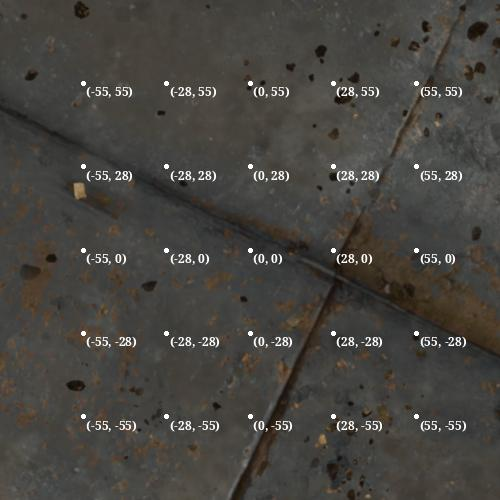
\includegraphics[width=0.5\linewidth]{images/GPT4o-CityNew-FS2/20_11.jpg}
    \end{center}
    
\gptspeaks: \( < \)Reasoning\( > \)I'll ascend to gain a better view and move to the northwest to locate a clear area.\( < \)/Reasoning\( > \)
\( < \)Action\( > \)(-28, 28, 10)\( < \)/Action\( > \)
\respeaks: Emergency stop; you've flown too close to something and would have hit it.
\respeaks: Your current altitude is 86 meters above ground level.
\StageDir{\re{} presents \gpt{} with a relevant image}

    \begin{center}
    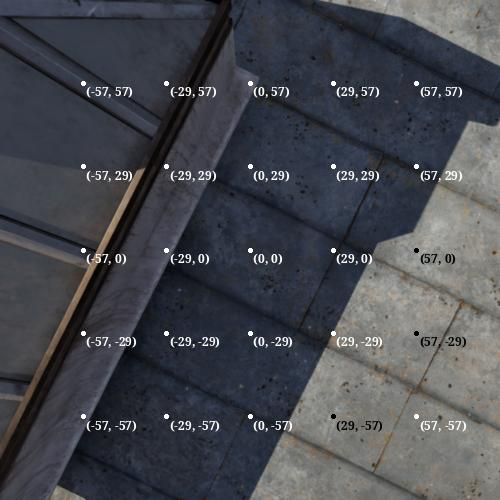
\includegraphics[width=0.5\linewidth]{images/GPT4o-CityNew-FS2/20_12.jpg}
    \end{center}
    
\gptspeaks: \( < \)Reasoning\( > \)I'll move southeast to avoid structures and try descending slightly to improve visibility of the area below.\( < \)/Reasoning\( > \)
\( < \)Action\( > \)(29, -29, -10)\( < \)/Action\( > \)
\respeaks: Emergency stop; you've flown too close to something and would have hit it.
\respeaks: Your current altitude is 83 meters above ground level.
\StageDir{\re{} presents \gpt{} with a relevant image}

    \begin{center}
    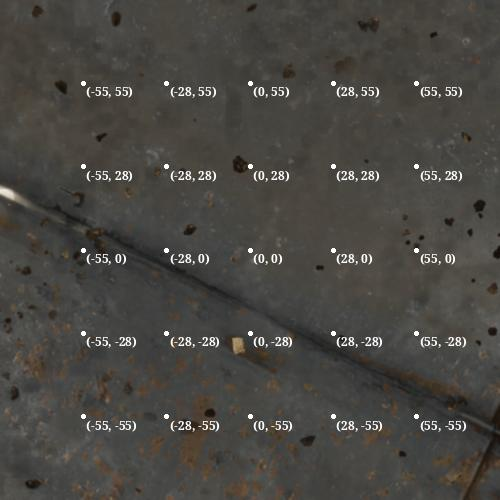
\includegraphics[width=0.5\linewidth]{images/GPT4o-CityNew-FS2/20_13.jpg}
    \end{center}
    
\gptspeaks: \( < \)Reasoning\( > \)I'll move to the east to avoid obstacles and try to descend slightly to get a clearer view.\( < \)/Reasoning\( > \)
\( < \)Action\( > \)(28, 0, -10)\( < \)/Action\( > \)
\respeaks: Emergency stop; you've flown too close to something and would have hit it.
\respeaks: Your current altitude is 83 meters above ground level.
\StageDir{\re{} presents \gpt{} with a relevant image}

    \begin{center}
    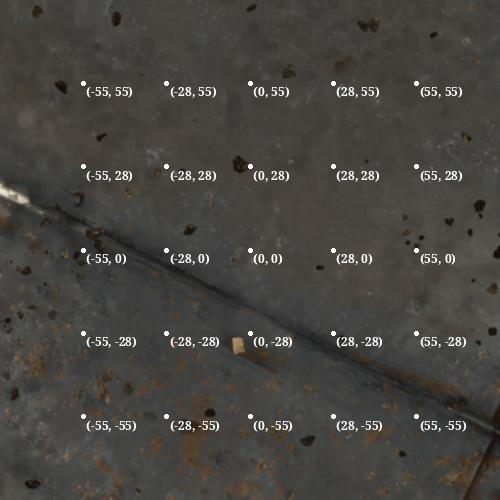
\includegraphics[width=0.5\linewidth]{images/GPT4o-CityNew-FS2/20_14.jpg}
    \end{center}
    
\gptspeaks: \( < \)Reasoning\( > \)I'll ascend to avoid obstacles and move to the northeast to find a clearer area.\( < \)/Reasoning\( > \)
\( < \)Action\( > \)(28, 28, 10)\( < \)/Action\( > \)
\respeaks: Your current altitude is 93 meters above ground level.
\StageDir{\re{} presents \gpt{} with a relevant image}

    \begin{center}
    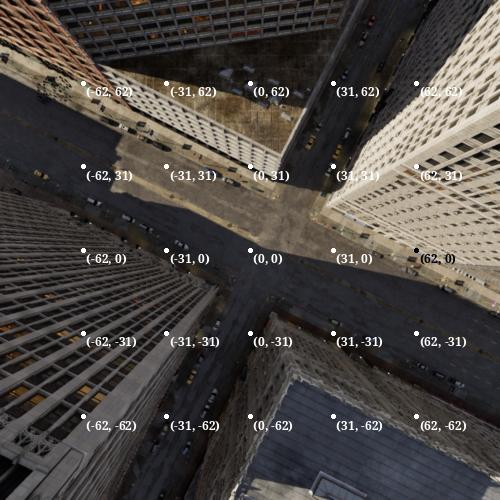
\includegraphics[width=0.5\linewidth]{images/GPT4o-CityNew-FS2/20_15.jpg}
    \end{center}
    
\gptspeaks: \( < \)Reasoning\( > \)The open area to the center of the intersection might provide a good view of the crowd. I'll move directly there and descend to get closer.\( < \)/Reasoning\( > \)
\( < \)Action\( > \)(0, 0, -40)\( < \)/Action\( > \)
\respeaks: Your current altitude is 53 meters above ground level.
\StageDir{\re{} presents \gpt{} with a relevant image}

    \begin{center}
    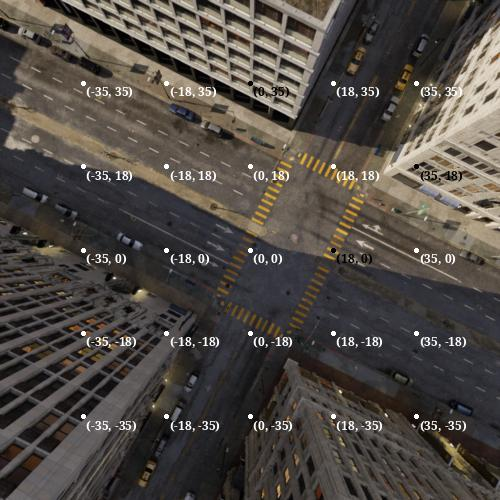
\includegraphics[width=0.5\linewidth]{images/GPT4o-CityNew-FS2/20_16.jpg}
    \end{center}
    
\gptspeaks: \( < \)Reasoning\( > \)I'll descend further and remain centered over the intersection to look for the crowd. This position should provide a clear view of the area.\( < \)/Reasoning\( > \)
\( < \)Action\( > \)(0, 0, -40)\( < \)/Action\( > \)
\respeaks: Your current altitude is 13 meters above ground level.
\StageDir{\re{} presents \gpt{} with a relevant image}

    \begin{center}
    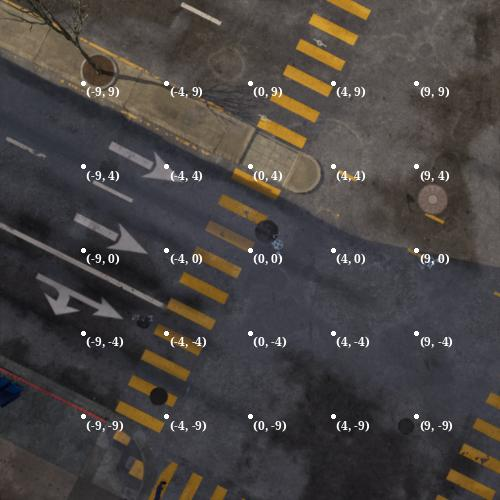
\includegraphics[width=0.5\linewidth]{images/GPT4o-CityNew-FS2/20_17.jpg}
    \end{center}
    
\gptspeaks: \( < \)Reasoning\( > \)I'm now close to the ground and centered over the intersection. I'll descend further to confirm the presence of the crowd.\( < \)/Reasoning\( > \)
\( < \)Action\( > \)(0, 0, -5)\( < \)/Action\( > \)
\respeaks: Your current altitude is 8 meters above ground level.
\StageDir{\re{} presents \gpt{} with a relevant image}

    \begin{center}
    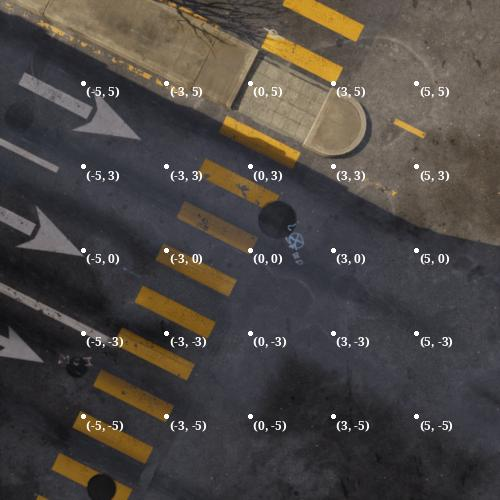
\includegraphics[width=0.5\linewidth]{images/GPT4o-CityNew-FS2/20_18.jpg}
    \end{center}
    
\gptspeaks: \( < \)Reasoning\( > \)I am now at an appropriate altitude and centered on the intersection, which matches the objective. I should confirm the presence of the crowd.\( < \)/Reasoning\( > \)
\( < \)Action\( > \)FOUND\( < \)/Action\( > \)
\end{drama}
\subsubsection{Example}

    \begin{itemize}[noitemsep,topsep=0pt]
      \item Starting position: (26.0, -106.0, 118.0)
      \item End position: (26.0, -116.0, 9.0) 
      \item Euclidean distance from the object: 119.21828718783037
      \item Object can be seen: False
      \item Success: False
      \item Object type: road construction site
      
    \end{itemize}
    

    \begin{center}
    \includegraphics[width=0.7\linewidth]{images/GPT4o-CityNew-FS2/21.pdf}
    \end{center}
    

    \begin{center}
    \includegraphics[width=0.7\linewidth]{images/GPT4o-CityNew-FS2/21_sit_awareness.pdf}
    \end{center}
    

    \begin{drama}
    \Character{Benchmark}{re}
    \Character{GPT-4o}{gpt}
    
\respeaks: \( < \)Context\( > \)
    You are in command of a UAV, tasked with finding road construction site.
\( < \)/Context\( > \) \texttt{(REST OF THE PROMPT)}
\respeaks: The object you're looking for is similar to this. This is NOT the drone's current view.
\StageDir{\re{} presents \gpt{} with a relevant image}

    \begin{center}
    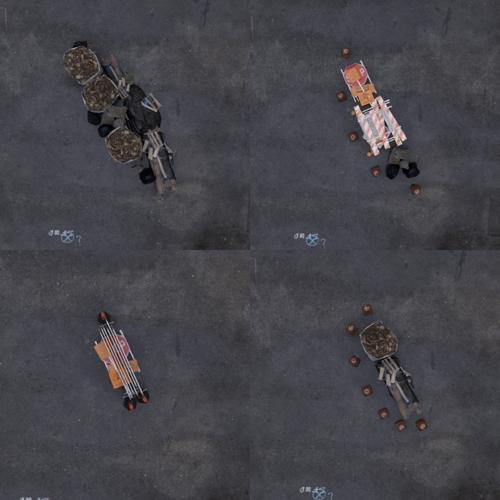
\includegraphics[width=0.5\linewidth]{images/GPT4o-CityNew-FS2/21_0.jpg}
    \end{center}
    
\respeaks: Your current altitude is 118 meters above ground level.
\StageDir{\re{} presents \gpt{} with a relevant image}

    \begin{center}
    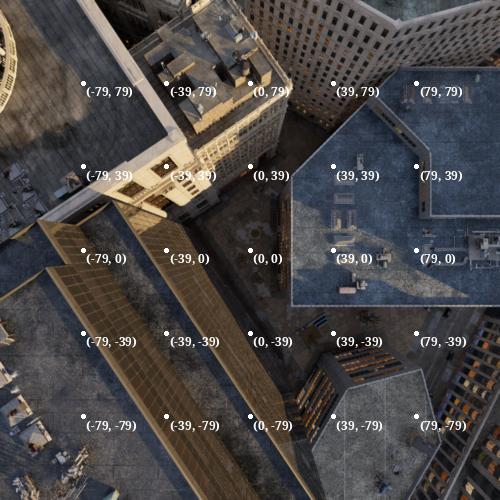
\includegraphics[width=0.5\linewidth]{images/GPT4o-CityNew-FS2/21_1.jpg}
    \end{center}
    
\gptspeaks: \( < \)Reasoning\( > \)The search area includes several grid points. I will start by moving to the nearest point that allows a better view of the area directly ahead. I'll descend to get closer to the potential object.\( < \)/Reasoning\( > \)
\( < \)Action\( > \)(0, 39, -30)\( < \)/Action\( > \)
\respeaks: Your current altitude is 88 meters above ground level.
\StageDir{\re{} presents \gpt{} with a relevant image}

    \begin{center}
    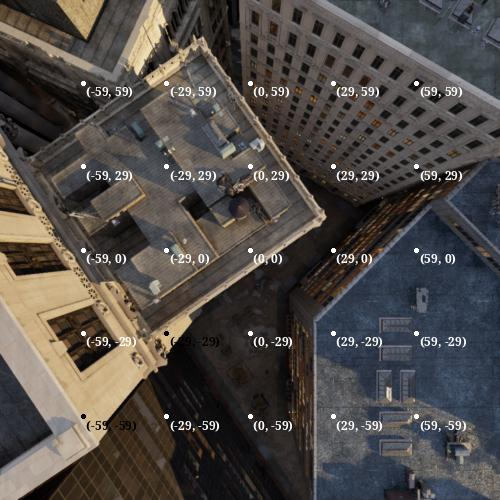
\includegraphics[width=0.5\linewidth]{images/GPT4o-CityNew-FS2/21_2.jpg}
    \end{center}
    
\gptspeaks: \( < \)Reasoning\( > \)I'll continue moving south to explore the lower area of the grid for better visibility, while also descending to get closer to the ground.\( < \)/Reasoning\( > \)
\( < \)Action\( > \)(0, -29, -30)\( < \)/Action\( > \)
\respeaks: Your current altitude is 58 meters above ground level.
\StageDir{\re{} presents \gpt{} with a relevant image}

    \begin{center}
    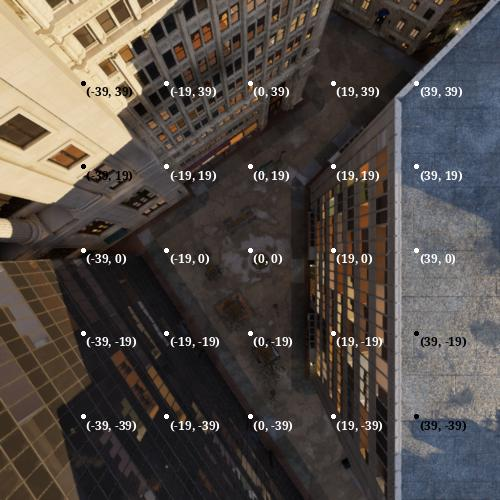
\includegraphics[width=0.5\linewidth]{images/GPT4o-CityNew-FS2/21_3.jpg}
    \end{center}
    
\gptspeaks: \( < \)Reasoning\( > \)The object might be in the open area below. I will move directly over the center of this area while continuing to descend to get a clearer view.\( < \)/Reasoning\( > \)
\( < \)Action\( > \)(0, 0, -30)\( < \)/Action\( > \)
\respeaks: Your current altitude is 28 meters above ground level.
\StageDir{\re{} presents \gpt{} with a relevant image}

    \begin{center}
    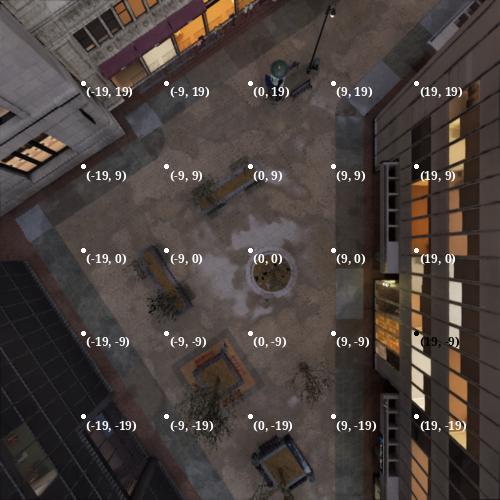
\includegraphics[width=0.5\linewidth]{images/GPT4o-CityNew-FS2/21_4.jpg}
    \end{center}
    
\gptspeaks: \( < \)Reasoning\( > \)The construction site is likely near the center of the open area. I'll continue to descend directly above it to ensure I'm within 10 meters.\( < \)/Reasoning\( > \)
\( < \)Action\( > \)(0, 0, -19)\( < \)/Action\( > \)
\respeaks: Your current altitude is 9 meters above ground level.
\StageDir{\re{} presents \gpt{} with a relevant image}

    \begin{center}
    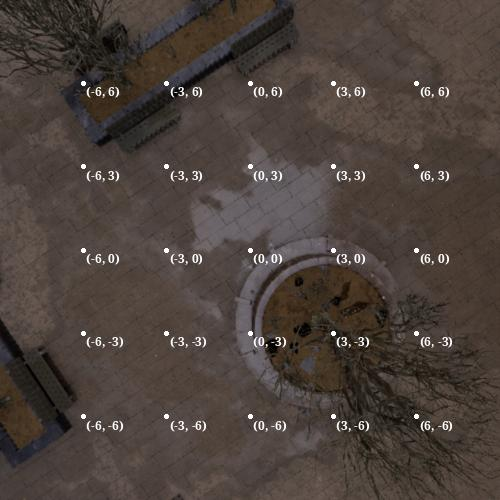
\includegraphics[width=0.5\linewidth]{images/GPT4o-CityNew-FS2/21_5.jpg}
    \end{center}
    
\gptspeaks: \( < \)Reasoning\( > \)I am now 9 meters above the object in the center of the image, which resembles the construction site. I am within 10 meters of altitude and centered over it.\( < \)/Reasoning\( > \)
\( < \)Answer\( > \)FOUND\( < \)/Answer\( > \)
\end{drama}
